\documentclass[11pt]{article}\usepackage[]{graphicx}\usepackage[]{xcolor}
% maxwidth is the original width if it is less than linewidth
% otherwise use linewidth (to make sure the graphics do not exceed the margin)
\makeatletter
\def\maxwidth{ %
  \ifdim\Gin@nat@width>\linewidth
    \linewidth
  \else
    \Gin@nat@width
  \fi
}
\makeatother

\definecolor{fgcolor}{rgb}{0.345, 0.345, 0.345}
\newcommand{\hlnum}[1]{\textcolor[rgb]{0.686,0.059,0.569}{#1}}%
\newcommand{\hlstr}[1]{\textcolor[rgb]{0.192,0.494,0.8}{#1}}%
\newcommand{\hlcom}[1]{\textcolor[rgb]{0.678,0.584,0.686}{\textit{#1}}}%
\newcommand{\hlopt}[1]{\textcolor[rgb]{0,0,0}{#1}}%
\newcommand{\hlstd}[1]{\textcolor[rgb]{0.345,0.345,0.345}{#1}}%
\newcommand{\hlkwa}[1]{\textcolor[rgb]{0.161,0.373,0.58}{\textbf{#1}}}%
\newcommand{\hlkwb}[1]{\textcolor[rgb]{0.69,0.353,0.396}{#1}}%
\newcommand{\hlkwc}[1]{\textcolor[rgb]{0.333,0.667,0.333}{#1}}%
\newcommand{\hlkwd}[1]{\textcolor[rgb]{0.737,0.353,0.396}{\textbf{#1}}}%
\let\hlipl\hlkwb

\usepackage{framed}
\makeatletter
\newenvironment{kframe}{%
 \def\at@end@of@kframe{}%
 \ifinner\ifhmode%
  \def\at@end@of@kframe{\end{minipage}}%
  \begin{minipage}{\columnwidth}%
 \fi\fi%
 \def\FrameCommand##1{\hskip\@totalleftmargin \hskip-\fboxsep
 \colorbox{shadecolor}{##1}\hskip-\fboxsep
     % There is no \\@totalrightmargin, so:
     \hskip-\linewidth \hskip-\@totalleftmargin \hskip\columnwidth}%
 \MakeFramed {\advance\hsize-\width
   \@totalleftmargin\z@ \linewidth\hsize
   \@setminipage}}%
 {\par\unskip\endMakeFramed%
 \at@end@of@kframe}
\makeatother

\definecolor{shadecolor}{rgb}{.97, .97, .97}
\definecolor{messagecolor}{rgb}{0, 0, 0}
\definecolor{warningcolor}{rgb}{1, 0, 1}
\definecolor{errorcolor}{rgb}{1, 0, 0}
\newenvironment{knitrout}{}{} % an empty environment to be redefined in TeX

\usepackage{alltt}

% Packages for graphics & layout
\usepackage{graphicx}
\usepackage{epstopdf}
\usepackage{caption}
\usepackage{subcaption}
\usepackage{booktabs}
\usepackage[a4paper,margin=0.5in]{geometry}
\usepackage{lipsum}

% Packages for math
\usepackage{amsmath}
\usepackage{amsfonts}
\usepackage{amssymb}

% Package for bibliography
\usepackage{natbib}
\usepackage{hyperref}


% listing setup
\usepackage{listings}
\usepackage{color} % For syntax highlighting color

\lstset{ 
  language=R,
  basicstyle=\small,
  commentstyle=\color{red},
  keywordstyle=\color{blue},
  numberstyle=\tiny\color{gray},
  stringstyle=\color{purple},
  breaklines=true,
  captionpos=b,
  keepspaces=true,
  numbers=left,
  numbersep=5pt,
  showspaces=false,
  showstringspaces=false,
  showtabs=false,
  tabsize=2
}

\captionsetup{labelfont=bf}
\setlength{\parskip}{0.5\baselineskip}


\title{Data Analysis Report}
\author{Michael V Cumbo}
\date{\today}
\IfFileExists{upquote.sty}{\usepackage{upquote}}{}
\begin{document}

\maketitle

\begin{abstract}
This document presents a comprehensive analysis of the data pertaining to trade unions.
\end{abstract}

\section{Introduction}
This paper was written in response to the United Auto Workers strike and the SAG-AFTRA strike of 2023. The goal of this paper is to contextualize the state of trade union power in the United States, blending data analysis with a literature review. The findings in this paper also contextualize union power in a select number of nation-states, adding perspective to the modes of influence individual working-class individuals may have within those states.

\section{Methodology}
\subsection*{Libraries Used in the Analysis}

This analysis utilized several R packages, each contributing unique functions essential for data management, manipulation, visualization, and database interaction. Below is a description of each package and its role in our analysis:

\begin{itemize}
    \item \textbf{tidyverse}: An aggregation of several data manipulation packages, \texttt{tidyverse} simplifies many aspects of data analysis. It includes packages like \texttt{ggplot2} for data visualization, \texttt{dplyr} for data manipulation, and \texttt{readr} for data import. Its unified data philosophy makes data science tasks more straightforward and efficient.
    \begin{itemize}
        \item Installation: \texttt{install.packages("tidyverse")}
        \item Documentation: \href{https://www.tidyverse.org/}{tidyverse.org}
    \end{itemize}
    
    \item \textbf{RSQLite}: This package provides a database interface and SQLite driver for R. It allows for seamless integration of SQLite database capabilities within R, enabling the storage, management, and retrieval of large datasets efficiently.
    \begin{itemize}
        \item Installation: \texttt{install.packages("RSQLite")}
        \item Documentation: \href{https://cran.r-project.org/web/packages/RSQLite/index.html}{RSQLite on CRAN}
    \end{itemize}
    
    \item \textbf{DBI}: The \texttt{DBI} package defines a common interface between R and database management systems. It is crucial for establishing database connections and executing database queries.
    \begin{itemize}
        \item Installation: \texttt{install.packages("DBI")}
        \item Documentation: \href{https://cran.r-project.org/web/packages/DBI/index.html}{DBI on CRAN}
    \end{itemize}
    
    \item \textbf{ggplot2}: A part of the \texttt{tidyverse}, \texttt{ggplot2} is a powerful and flexible tool for creating elegant data visualizations in R. It is based on the Grammar of Graphics and allows for building plots iteratively.
    \begin{itemize}
        \item Installation: \texttt{install.packages("ggplot2")}
        \item Documentation: \href{https://ggplot2.tidyverse.org/}{ggplot2.tidyverse.org}
    \end{itemize}
    
    \item \textbf{dplyr}: Also within the \texttt{tidyverse}, \texttt{dplyr} is used for data manipulation. It provides a set of verbs like filter, select, mutate, and summarize, making data manipulation tasks more intuitive and readable.
    \begin{itemize}
        \item Installation: \texttt{install.packages("dplyr")}
        \item Documentation: \href{https://dplyr.tidyverse.org/}{dplyr.tidyverse.org}
    \end{itemize}
    
    \item \textbf{forcats}: This package, part of the \texttt{tidyverse}, is designed for handling categorical variables (factors in R). It provides functions for reordering factor levels, collapsing levels, and changing the display of factor levels.
    \begin{itemize}
        \item Installation: \texttt{install.packages("forcats")}
        \item Documentation: \href{https://forcats.tidyverse.org/}{forcats.tidyverse.org}
    \end{itemize}
    
    \item \textbf{GGally}: An extension of \texttt{ggplot2}, \texttt{GGally} provides additional functions and utilities to enhance the capability of \texttt{ggplot2}, especially for creating complex multi-plot layouts.
    \begin{itemize}
        \item Installation: \texttt{install.packages("GGally")}
        \item Documentation: \href{https://cran.r-project.org/web/packages/GGally/index.html}{GGally on CRAN}
    \end{itemize}
    
    \item \textbf{stringr}: This package, also a part of the \texttt{tidyverse}, simplifies the process of working with strings (text data). It provides consistent and easy-to-use functions for string manipulation.
    \begin{itemize}
        \item Installation: \texttt{install.packages("stringr")}
        \item Documentation: \href{https://stringr.tidyverse.org/}{stringr.tidyverse.org}
    \end{itemize}
\end{itemize}

These libraries collectively provided the comprehensive toolkit necessary for our data analysis, from data manipulation and querying to visualization and string processing.

\subsection{Data Collection}
Data was sourced from the International Labor Organization, OECD datasets, and Harvard datasets.

\subsection{Data Preparation}
Data was sourced from the appropiate online databases and stored into a SQLite database. The data cleaning required the changing of column names to make the data more readable. Data was extracted from the databases into a tibble and prepared to be analysed using the following code: 
\begin{lstlisting}{language=R}
# R code snippet
setwd("~/workbook")
con <- dbConnect(RSQLite::SQLite(), "trade_union_data.db")
dbListTables(con)
tudr <- as_tibble(dbReadTable(con, "TUDR"))
cbcr <- as_tibble(dbReadTable(con, "CBCR"))
collective_bargaining <- as_tibble(dbReadTable(con, "CollectiveBargaining"))
trade_union_density <- as_tibble(dbReadTable(con, "TradeUnionDensity"))
workplace_rights <- as_tibble(dbReadTable(con, "WorkplaceRights"))
state_union_membership_density <-
  as_tibble(dbReadTable(con, "State_Union_Membership_Density_1964-2021"))
dbDisconnect(con)
\end{lstlisting}



\begin{figure}[h]
\centering
  \begin{minipage}{0.7\linewidth}
  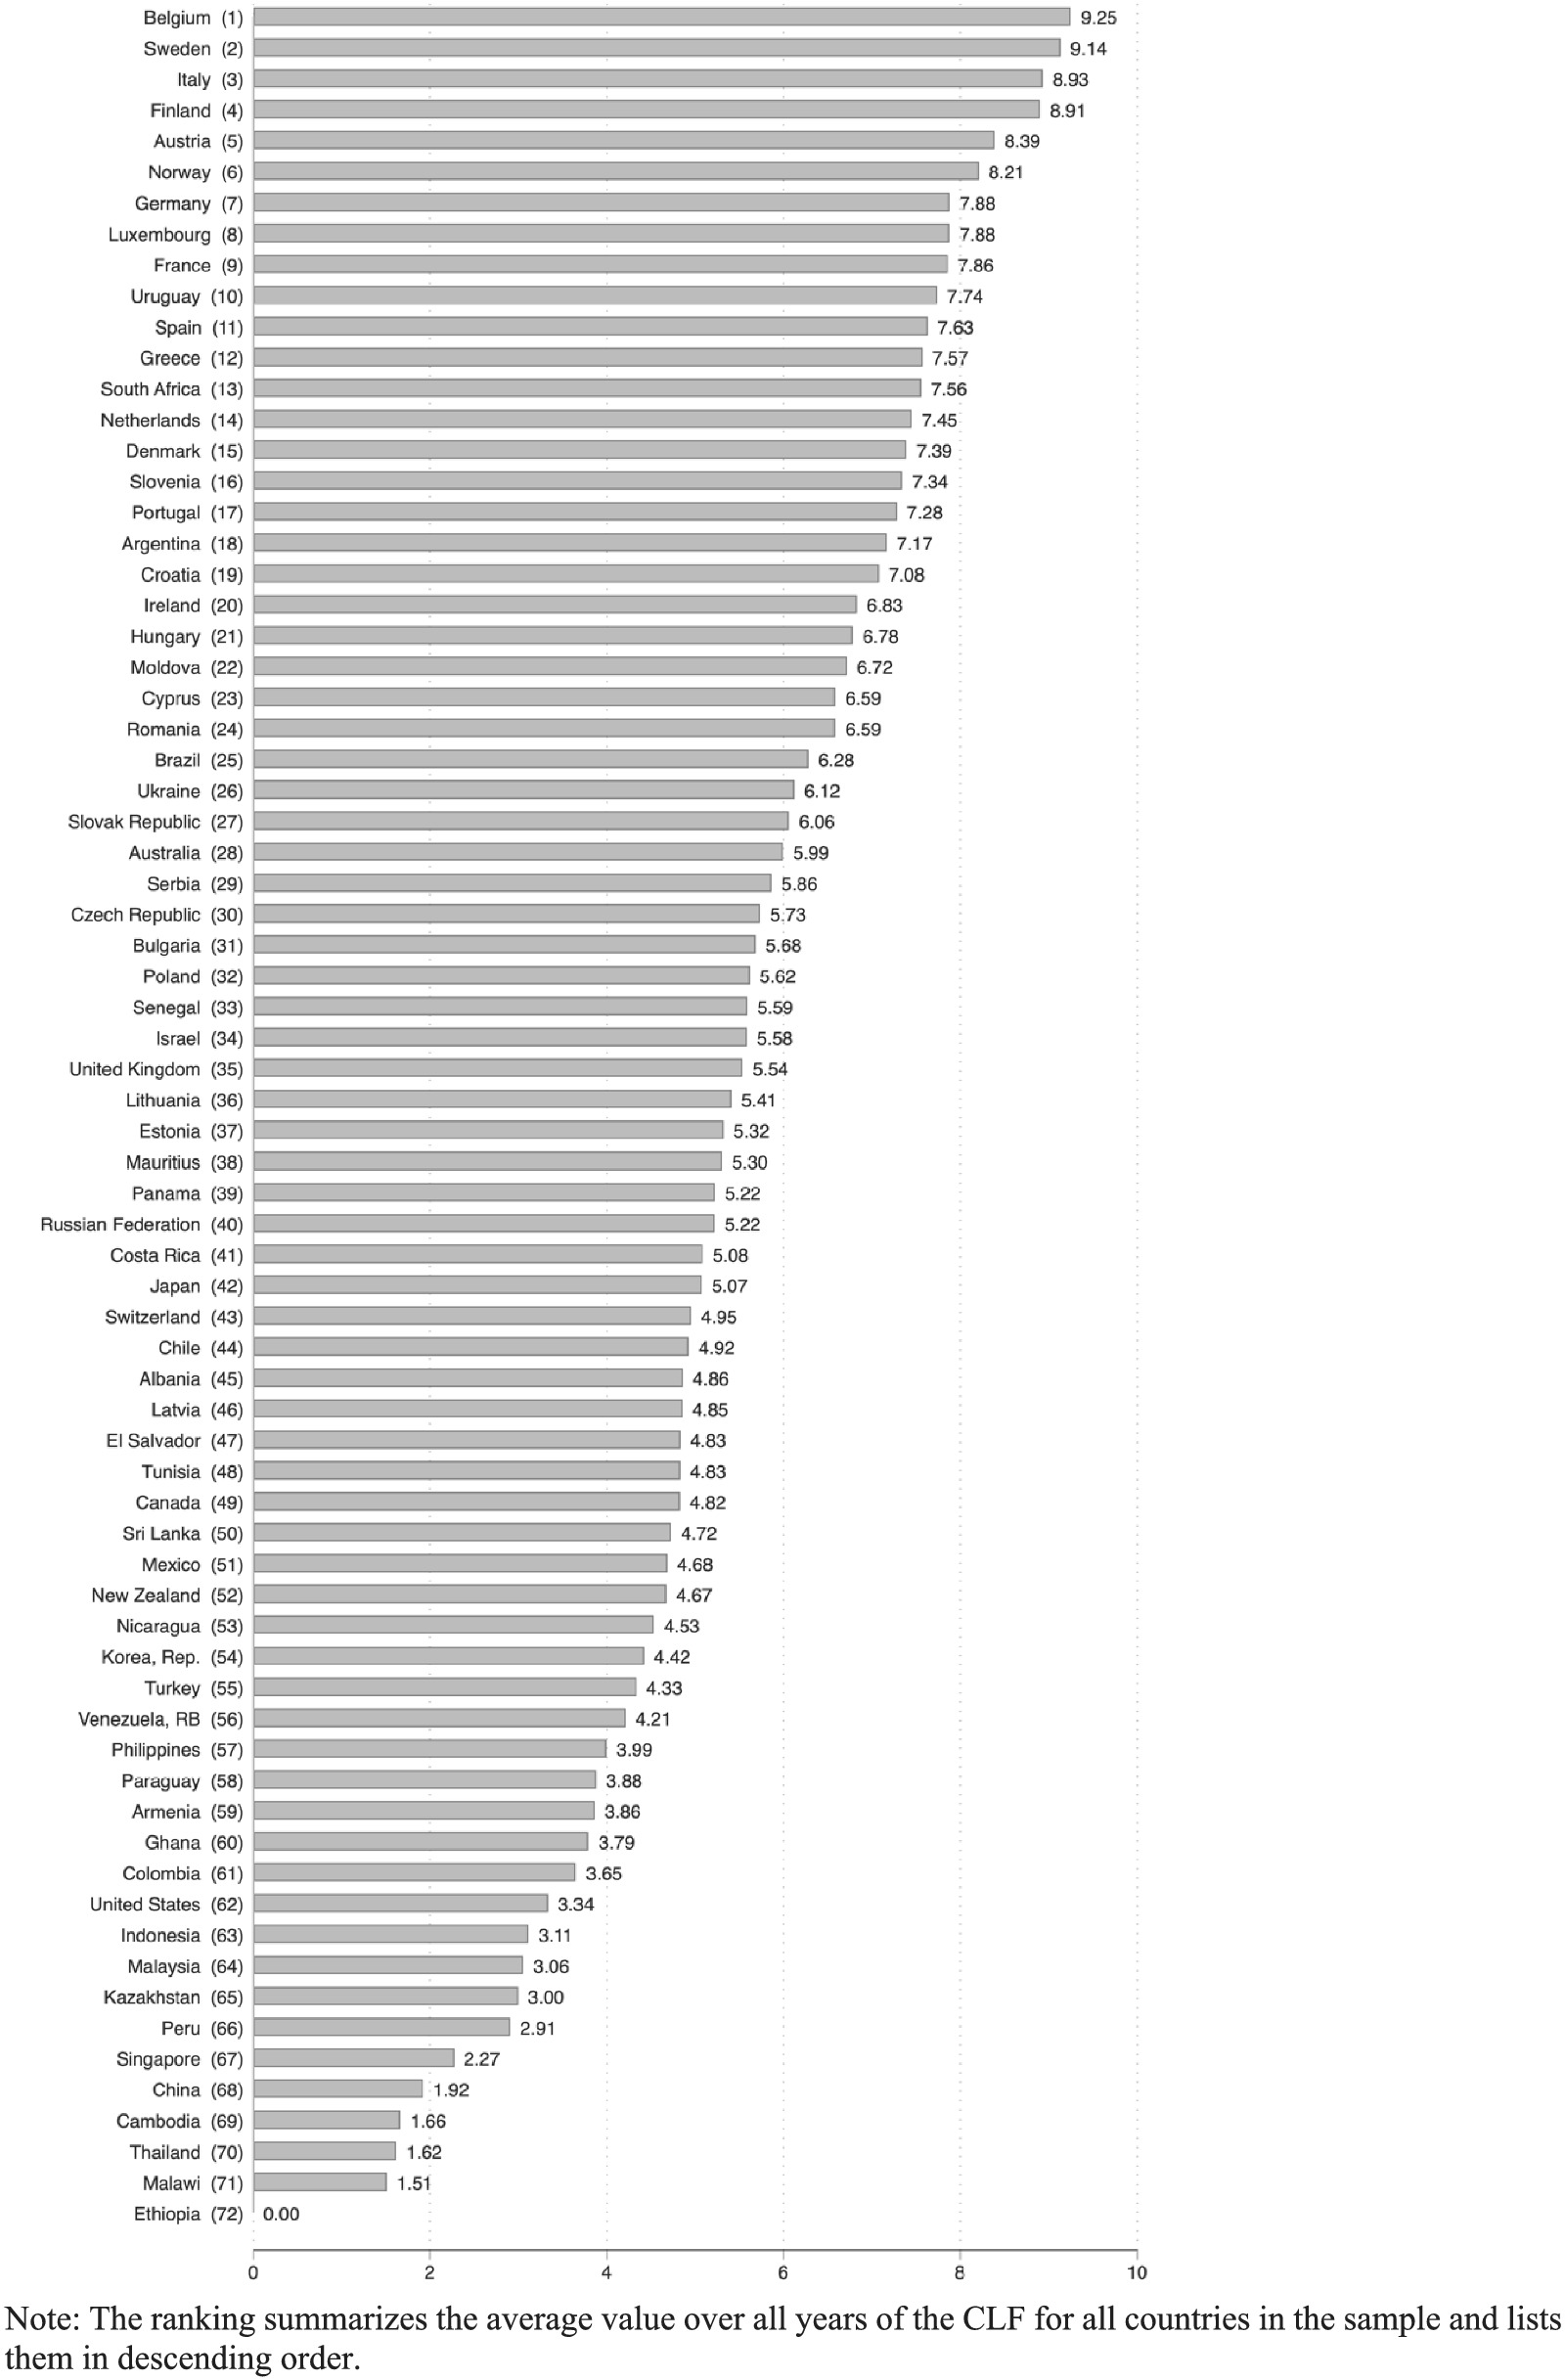
\includegraphics[width=\linewidth]{~/Lab2/graphs/udstudfy.jpg}
  \caption{Histogram depicting the distribution of the collective labour force index. The incomplete data availability pushes the Index down to around 72 countries, so the ranking matters less than the Index itself. The picture it paints is the freedom a working person has in the labor force(Union Power). This study is an assessment of union power. It indicates union power by combining and weighing the following stats: Trade Union Density, Collective Bargaining Coverage, Labour Force Participation Rate, Employment in agriculture, Democracy, Core labor rights ratification, hiring and firing constraints, and Hours Regulation. The United States is 62(3.32 index rating) in the Index, and China's place is 68 (1.92 index rating). The data is only recorded from 2010 to 2016. }
  \label{fig:1.0}
  \end{minipage}
\end{figure}
\footnotetext{Source: Metten, A. (2021). \textit{Rethinking Trade Union Density: A new index for Measuring Union Strength.}Industrial Relations Journal, 52(6), 528–549. https://doi.org/10.1111/irj.12347}


\clearpage
\section{Discussion}
For the United States, it is essential to note that the 2020s have seen a growing labor movement, a slow but consistent growth in strikes and labor action, which typically leads to increases in labor union density and collective bargaining coverage (see West Virginia in the 1970s as shown in figure~\ref{fig:1.3}, which saw a sharp increase of ten percent union membership due to wildcat strikes). Because of this, there is a strong possibility that the quality of life could improve greatly for working-class people in the US at the end of this decade. 

China, when breaking down the stats, has a density of forty percent; however, there is only one union that exists in China, the All-China Federation of Trade Unions (ACFTU), a state-controlled union that allows company chiefs to elect the leadership of the union. It is not really a union, as it is an apparatus of state control. So, things like strikes and collective bargaining agreements are off the table for your average Chinese citizen. See this book for more details on how the ACFTU operates:  Fu, Diana (2017). Mobilizing Without the Masses: \href{https://www.amazon.com/Mobilizing-without-Masses-Contention-Contentious/dp/1108430414}{Control and Contention in China. Cambridge University Press.}

Unions, and thus the quality of life in the United States, have been decreasing over the past 50 years. The US, for the first time in a century, has a National Labour Relations Board that is \href {https://www.theguardian.com/us-news/2023/sep/02/union-nlrb-decision-delays-busting}{friendly toward unions} There are things to look forward to coming to the US(including but not limited to a maglev \href{https://northeastmaglev.com/project/}{connecting Baltimore to New York and DC}. ), and the more active our unions get, the better our quality of life will get. China, however, doesn't have access to mechanisms that can truly redistribute wealth as it is created. Even if the ACFTU wanted to, it would be up to what the company chiefs allow. 




\begin{figure}[h]
\centering
  \begin{minipage}{0.9\linewidth}
  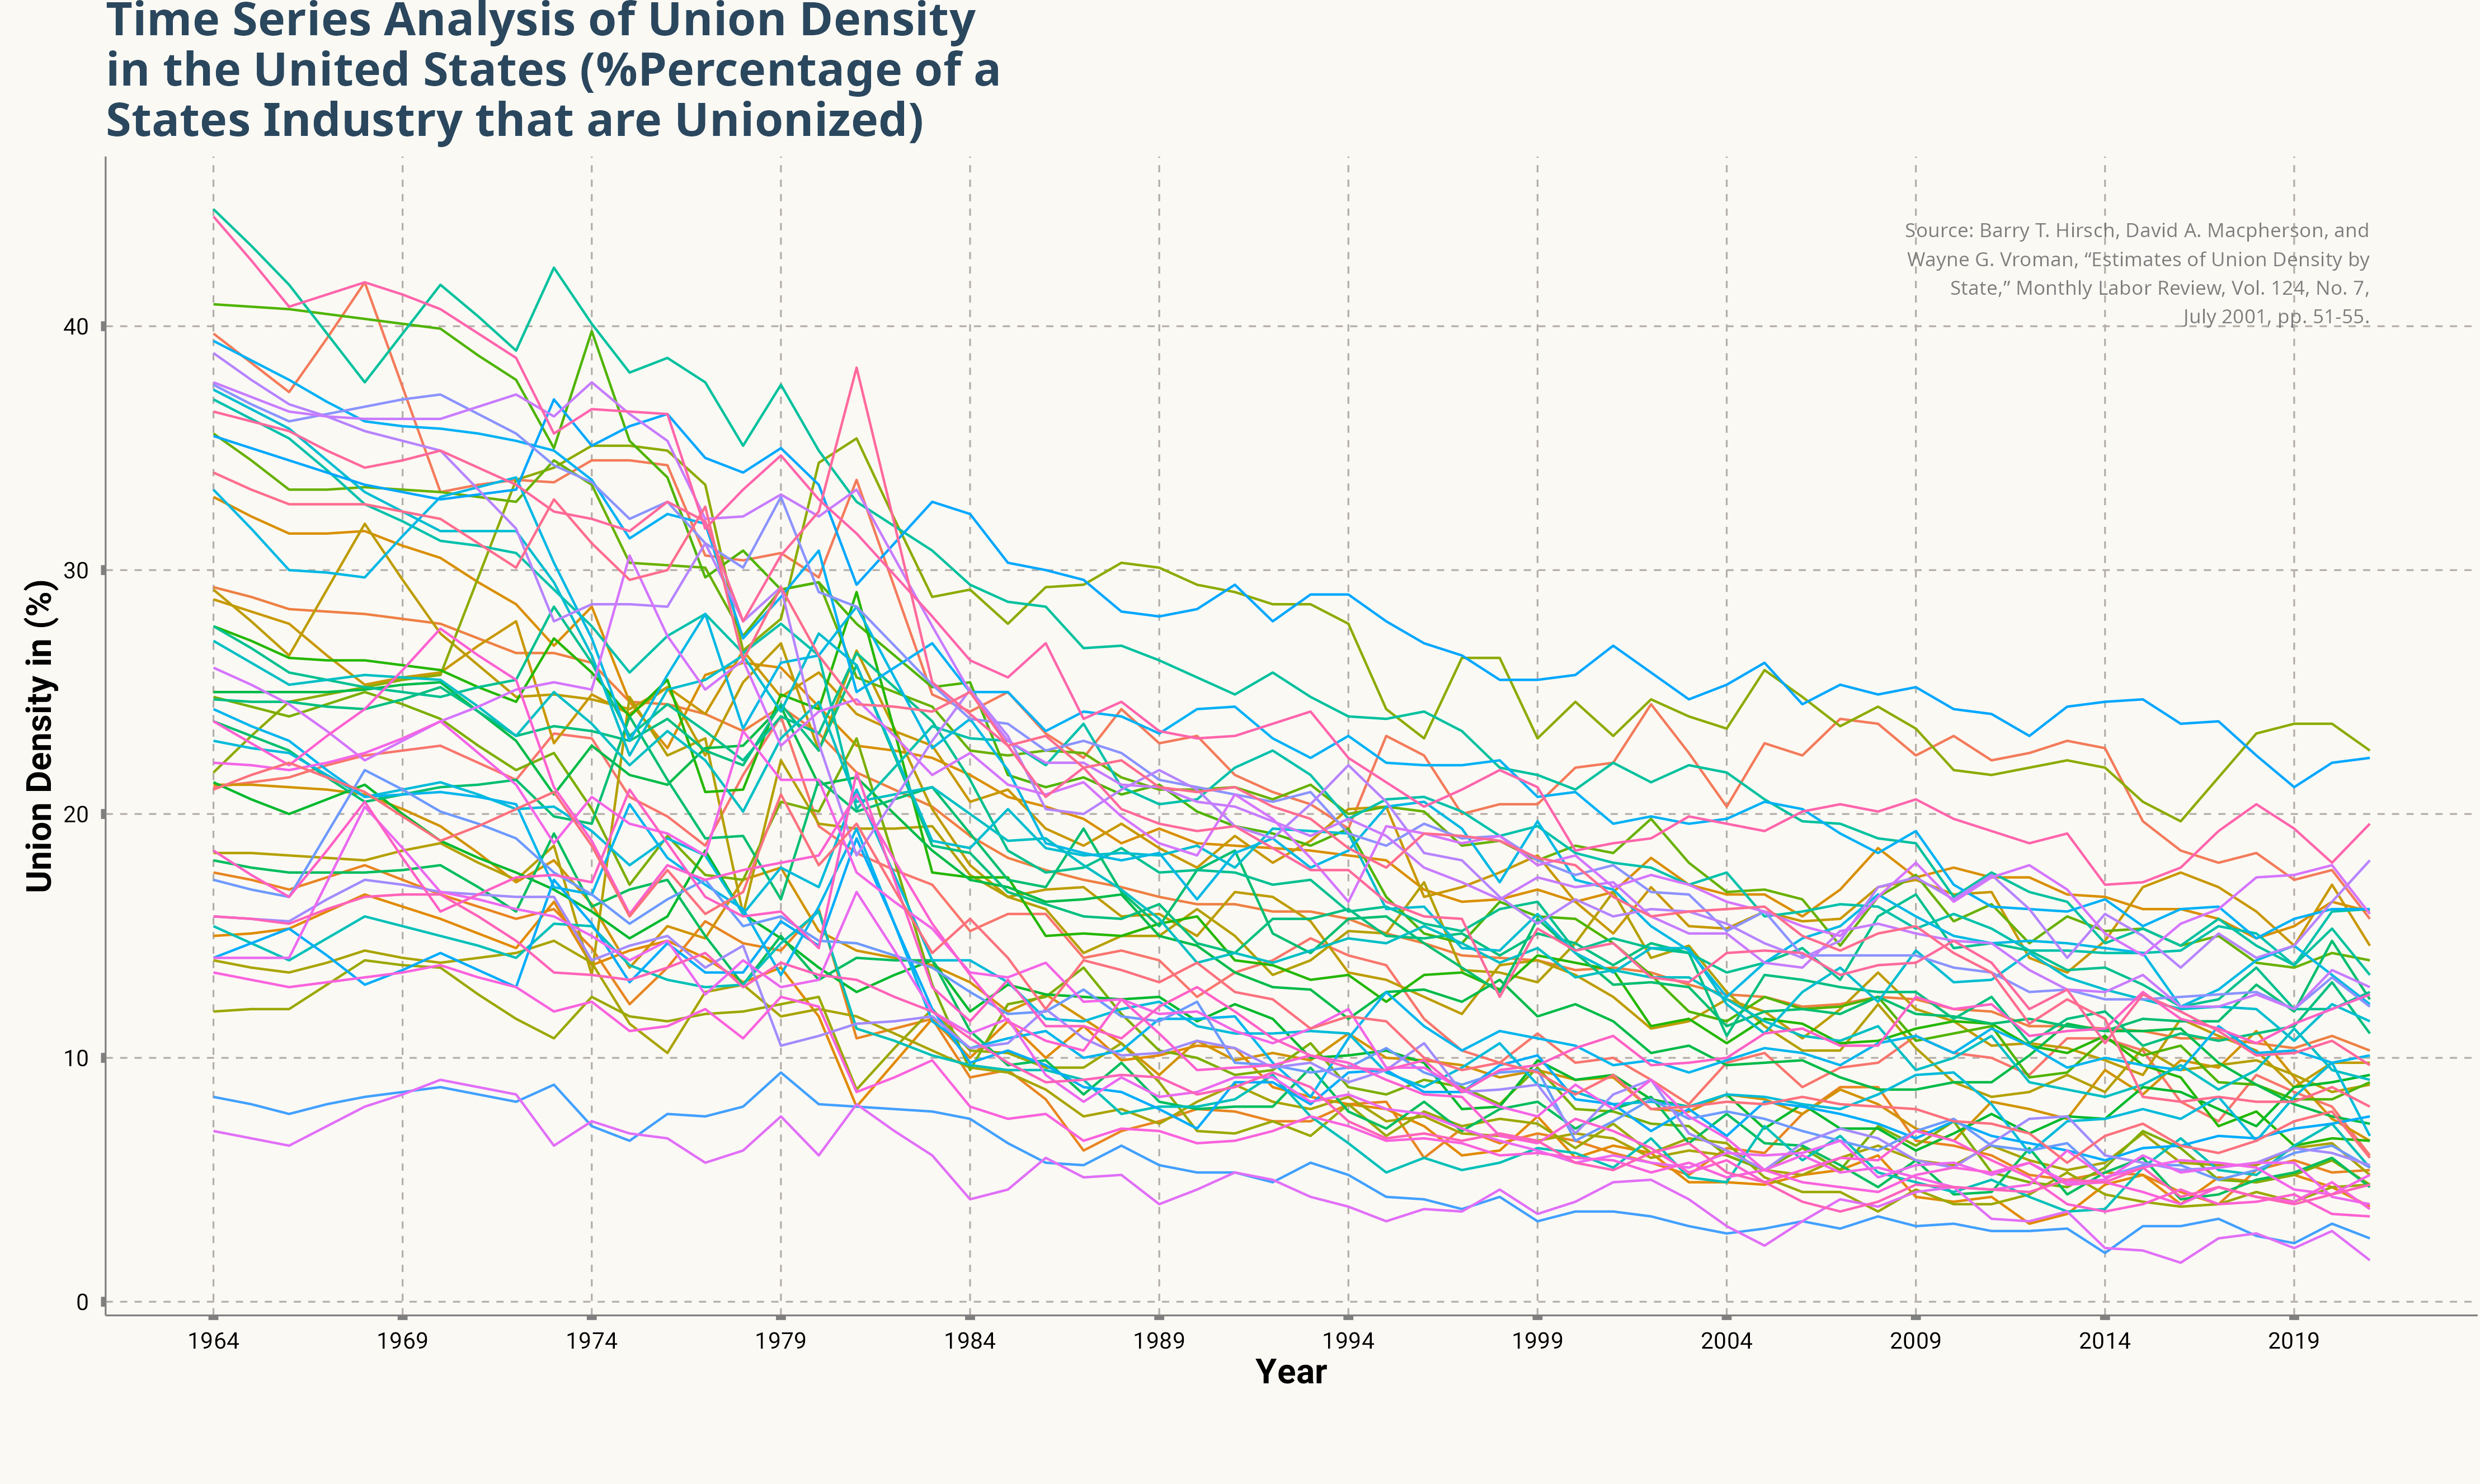
\includegraphics[width=\linewidth]{~/Lab2/graphs/plot_10.png}
  \caption{[Detailed caption for Figure 1]}
  \label{fig:1.1}
  \end{minipage}
\end{figure}

\begin{figure}[h]
\centering
\begin{minipage}{0.9\linewidth}
  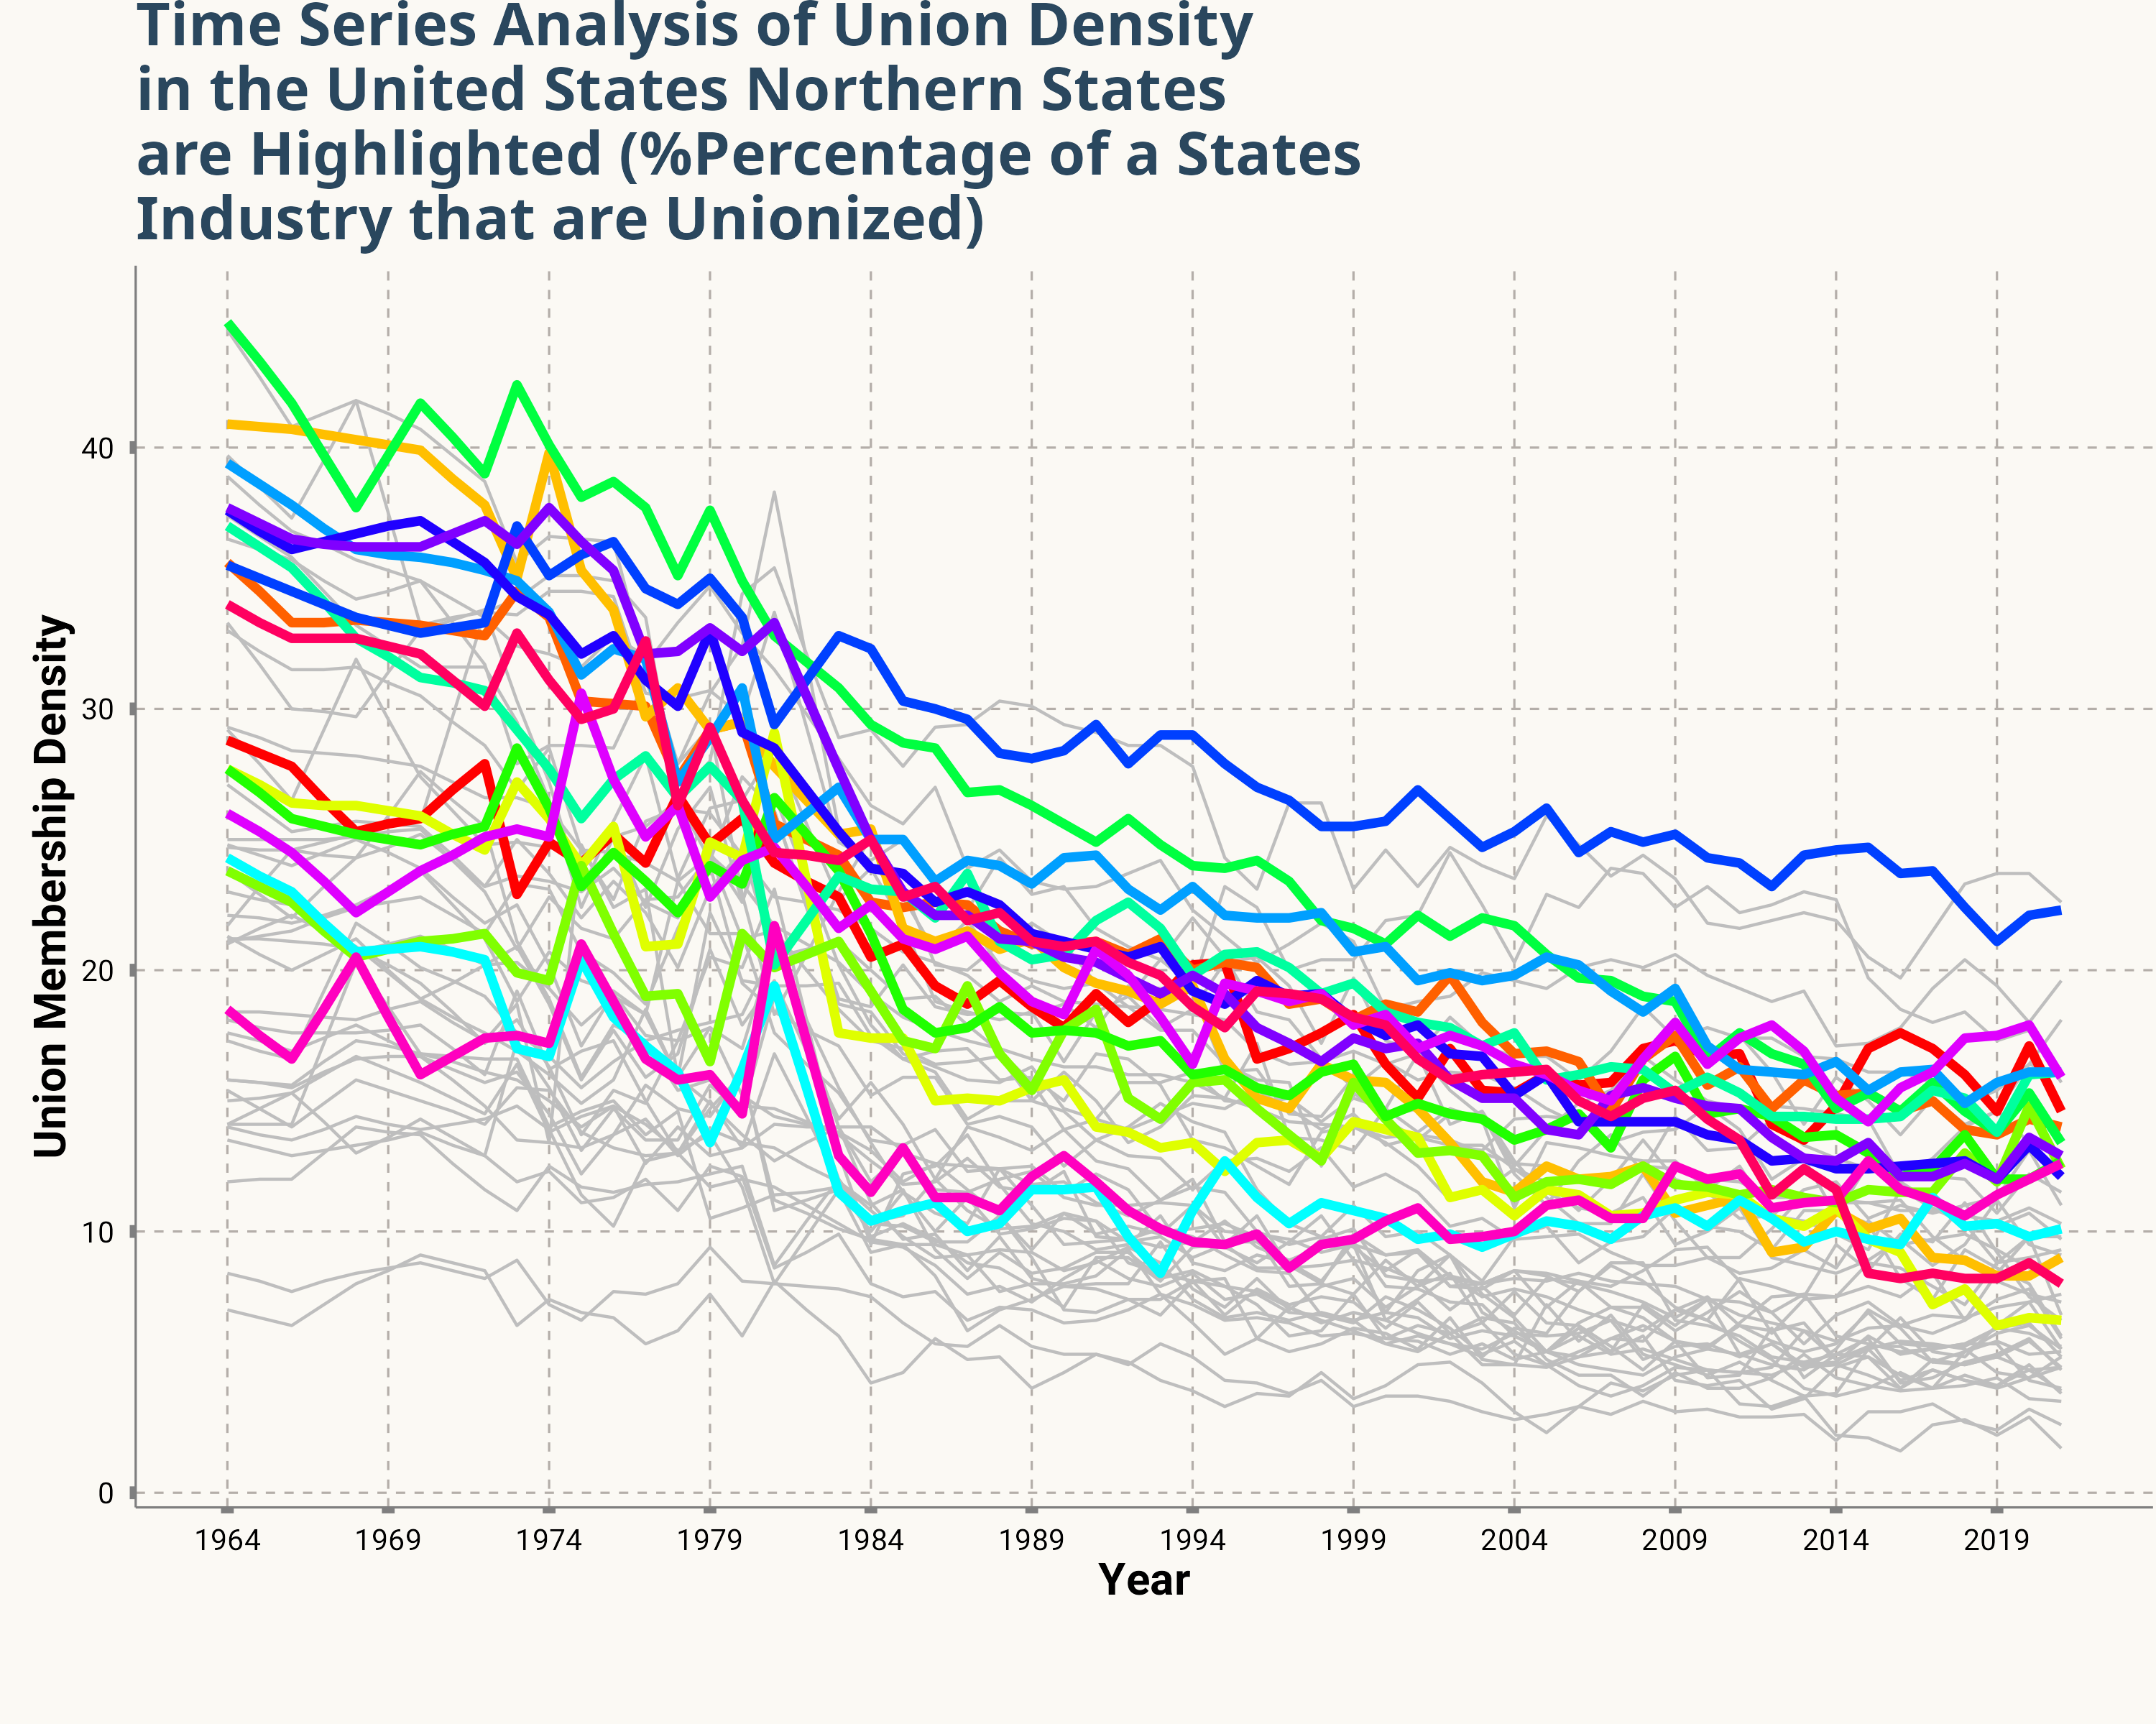
\includegraphics[width=\linewidth]{~/Lab2/graphs/plot_11.png}
  \caption{[Detailed caption for Figure 2]}
  \label{fig:1.2}
  \end{minipage}
\end{figure}

\begin{figure}[h]
\centering
\begin{minipage}{0.9\linewidth}
  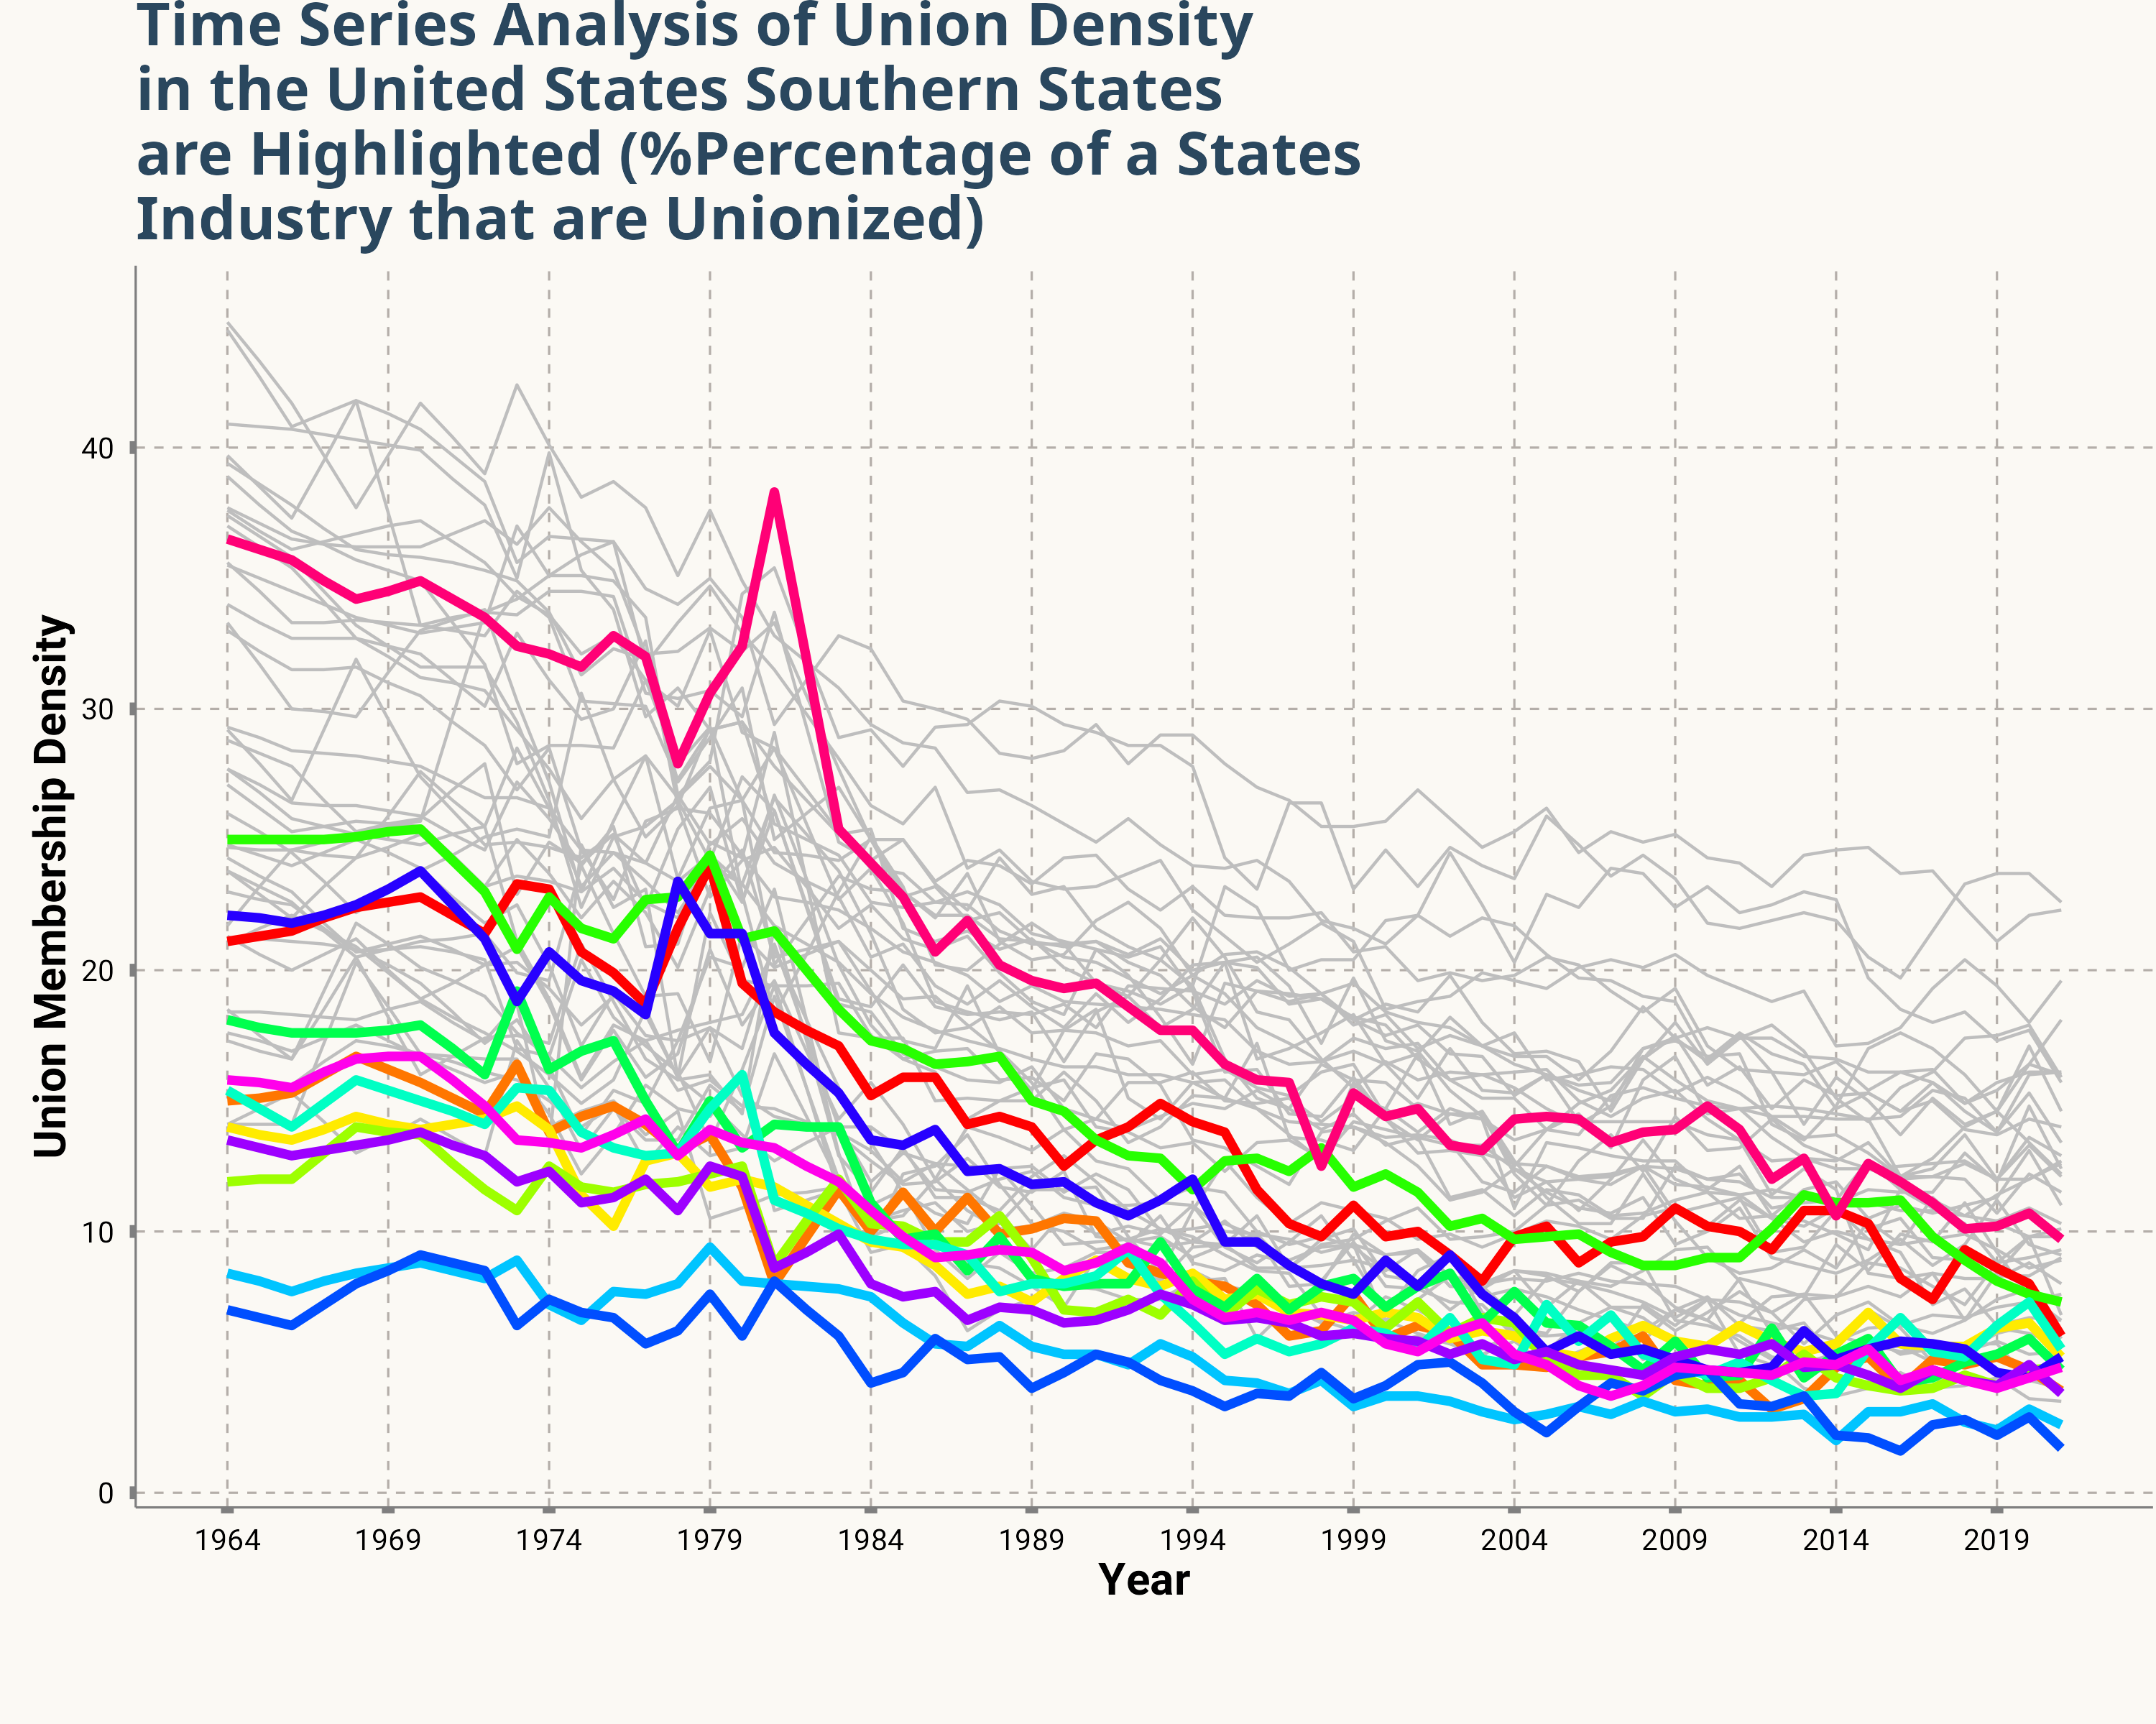
\includegraphics[width=\linewidth]{~/Lab2/graphs/plot_12.png}
  \caption{[Detailed caption for Figure 3]}
  \label{fig:1.3}
  \end{minipage}
\end{figure}

\begin{figure}[h]
\centering
\begin{minipage}{0.7\linewidth}
  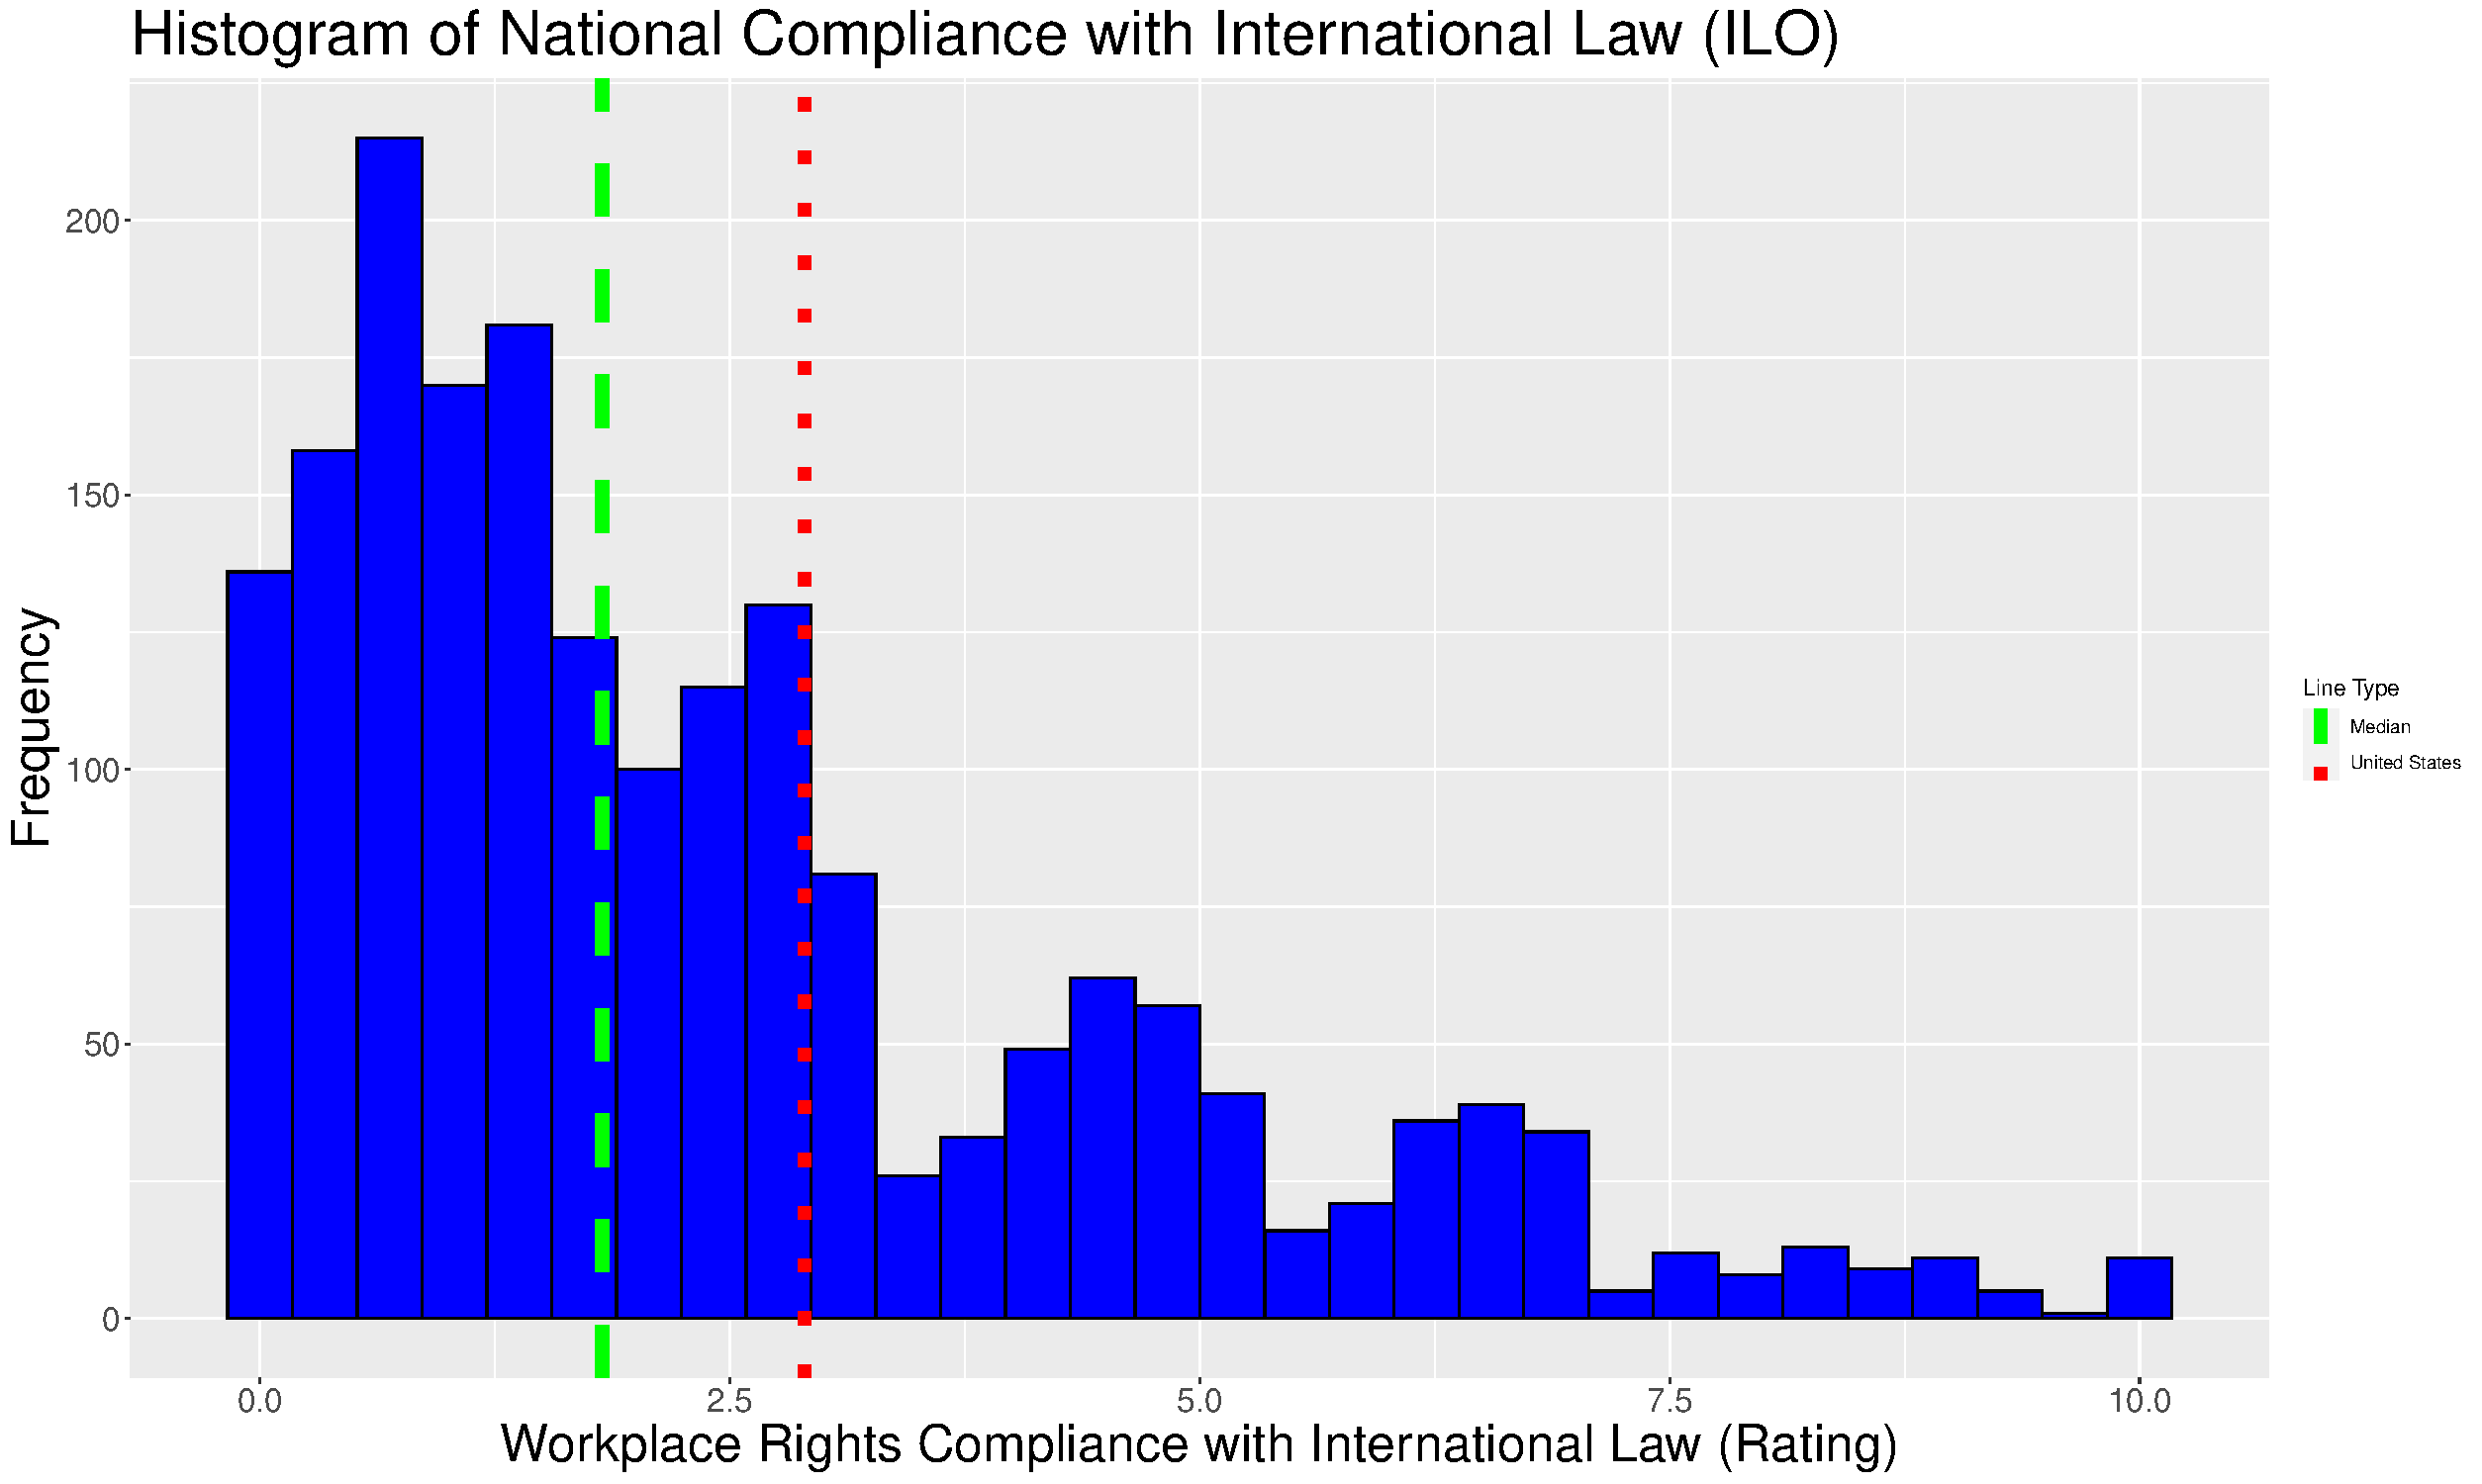
\includegraphics[width=.9\textwidth]{~/Lab2/graphs/plot_8.pdf}
  \caption[Collective Bargaining Coverage]{\textbf {Collective Bargaining Coverage 2000-2019} Histogram depicting the frequency distribution of collective bargaining coverage measured in percent recorded by the International Labor Organization database. The data is grouped by country, highlighting the predominance of collective bargaining coverage in the United States compared to the rest of the world.}
  \label{fig:2.1}
  \end{minipage}
\end{figure}

\begin{figure}[h]
\centering
  \begin{minipage}{0.7\linewidth}
  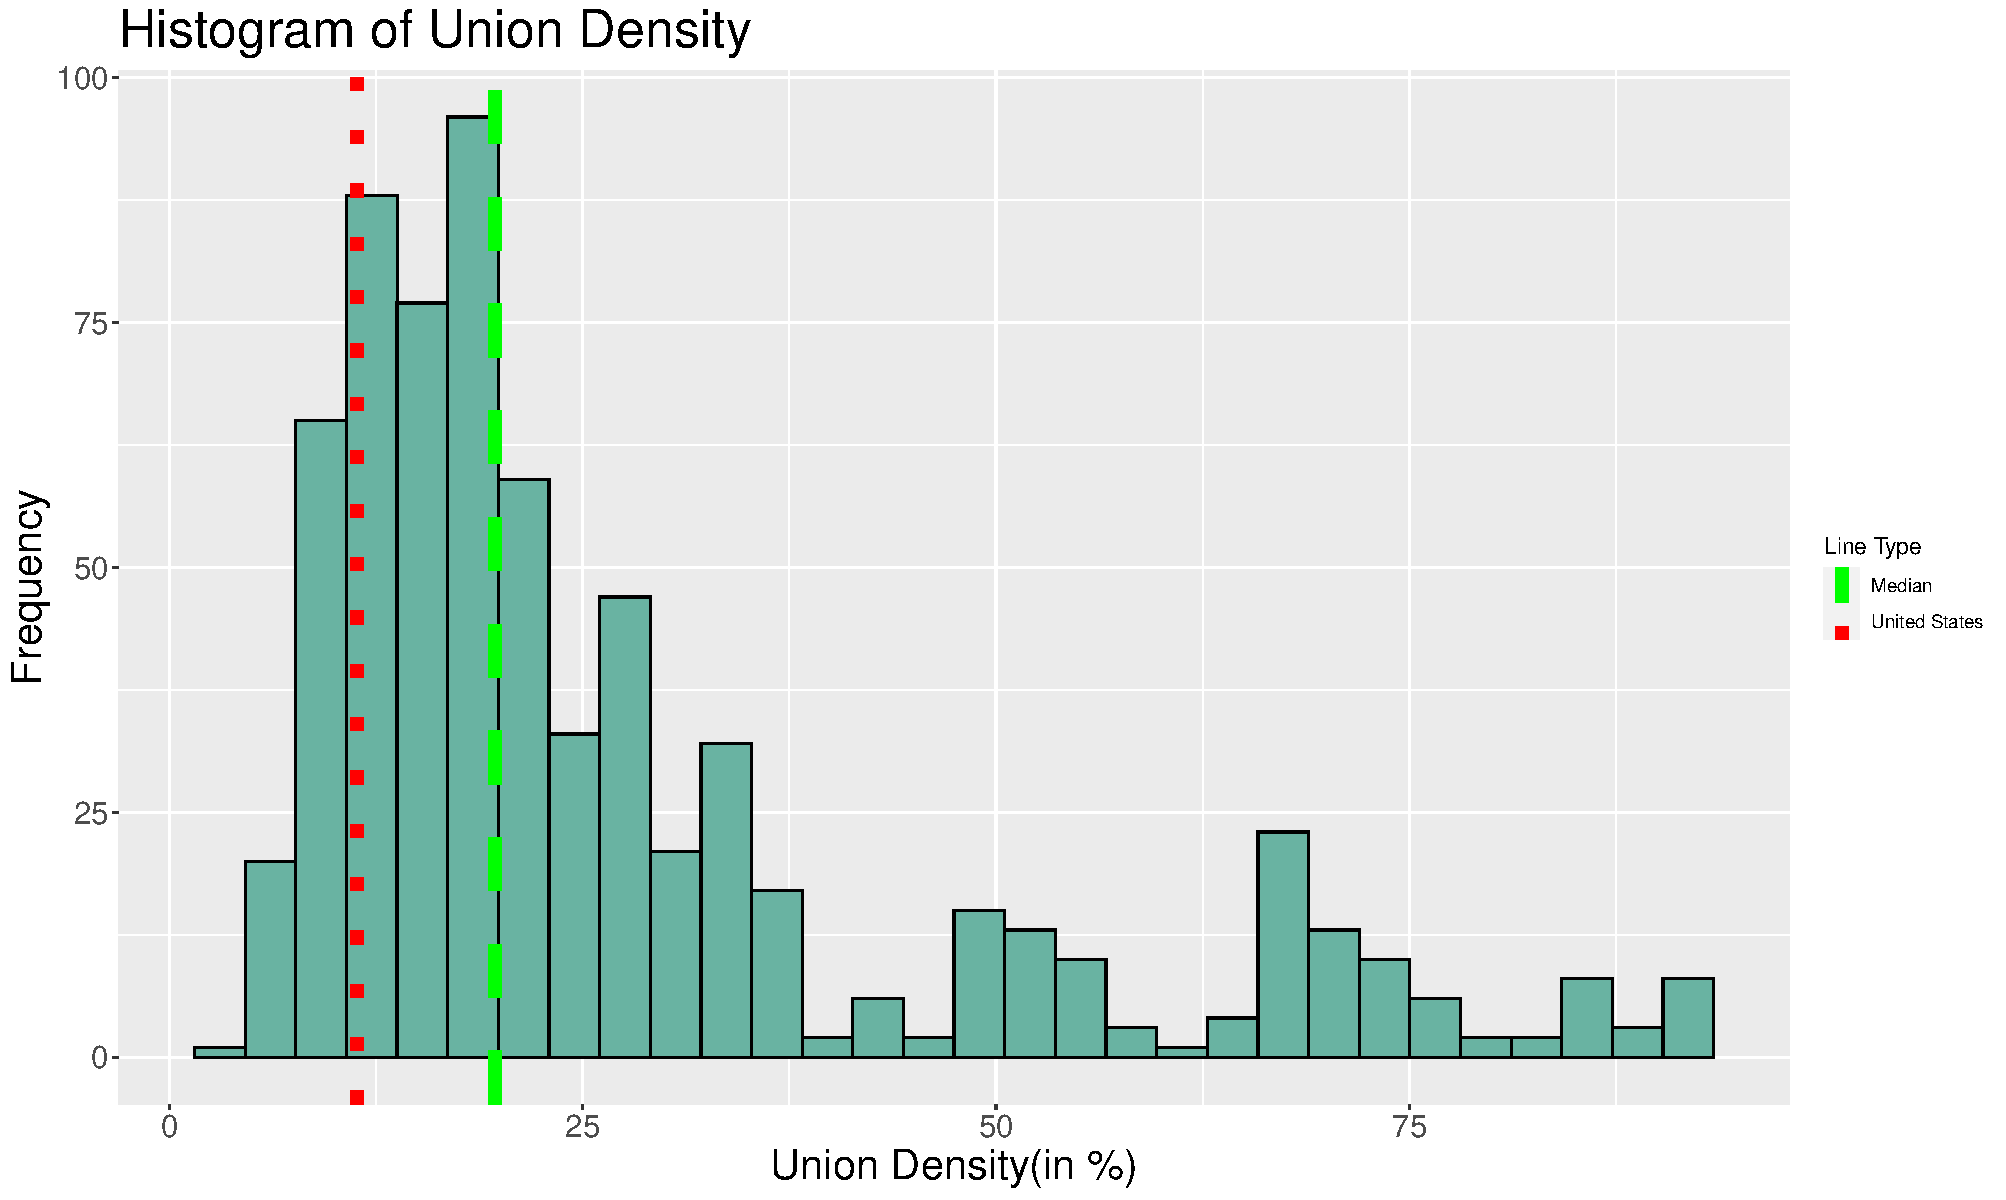
\includegraphics[width=.9\textwidth]{~/Lab2/graphs/plot_8-1.pdf}
  \caption{Histogram depicting the frequency distribution of Union Density in percent. The percentage measures a country's total unionized industries; the higher the percentage, the more of that country's workforce is unionized. This data is grouped by country; the mean of the United States and the mean of the total population are marked on this graph.} 
  \label{fig:2.2}
  \end{minipage}
\end{figure}

\begin{figure}[h]
\centering
  \begin{minipage}{0.7\linewidth}
  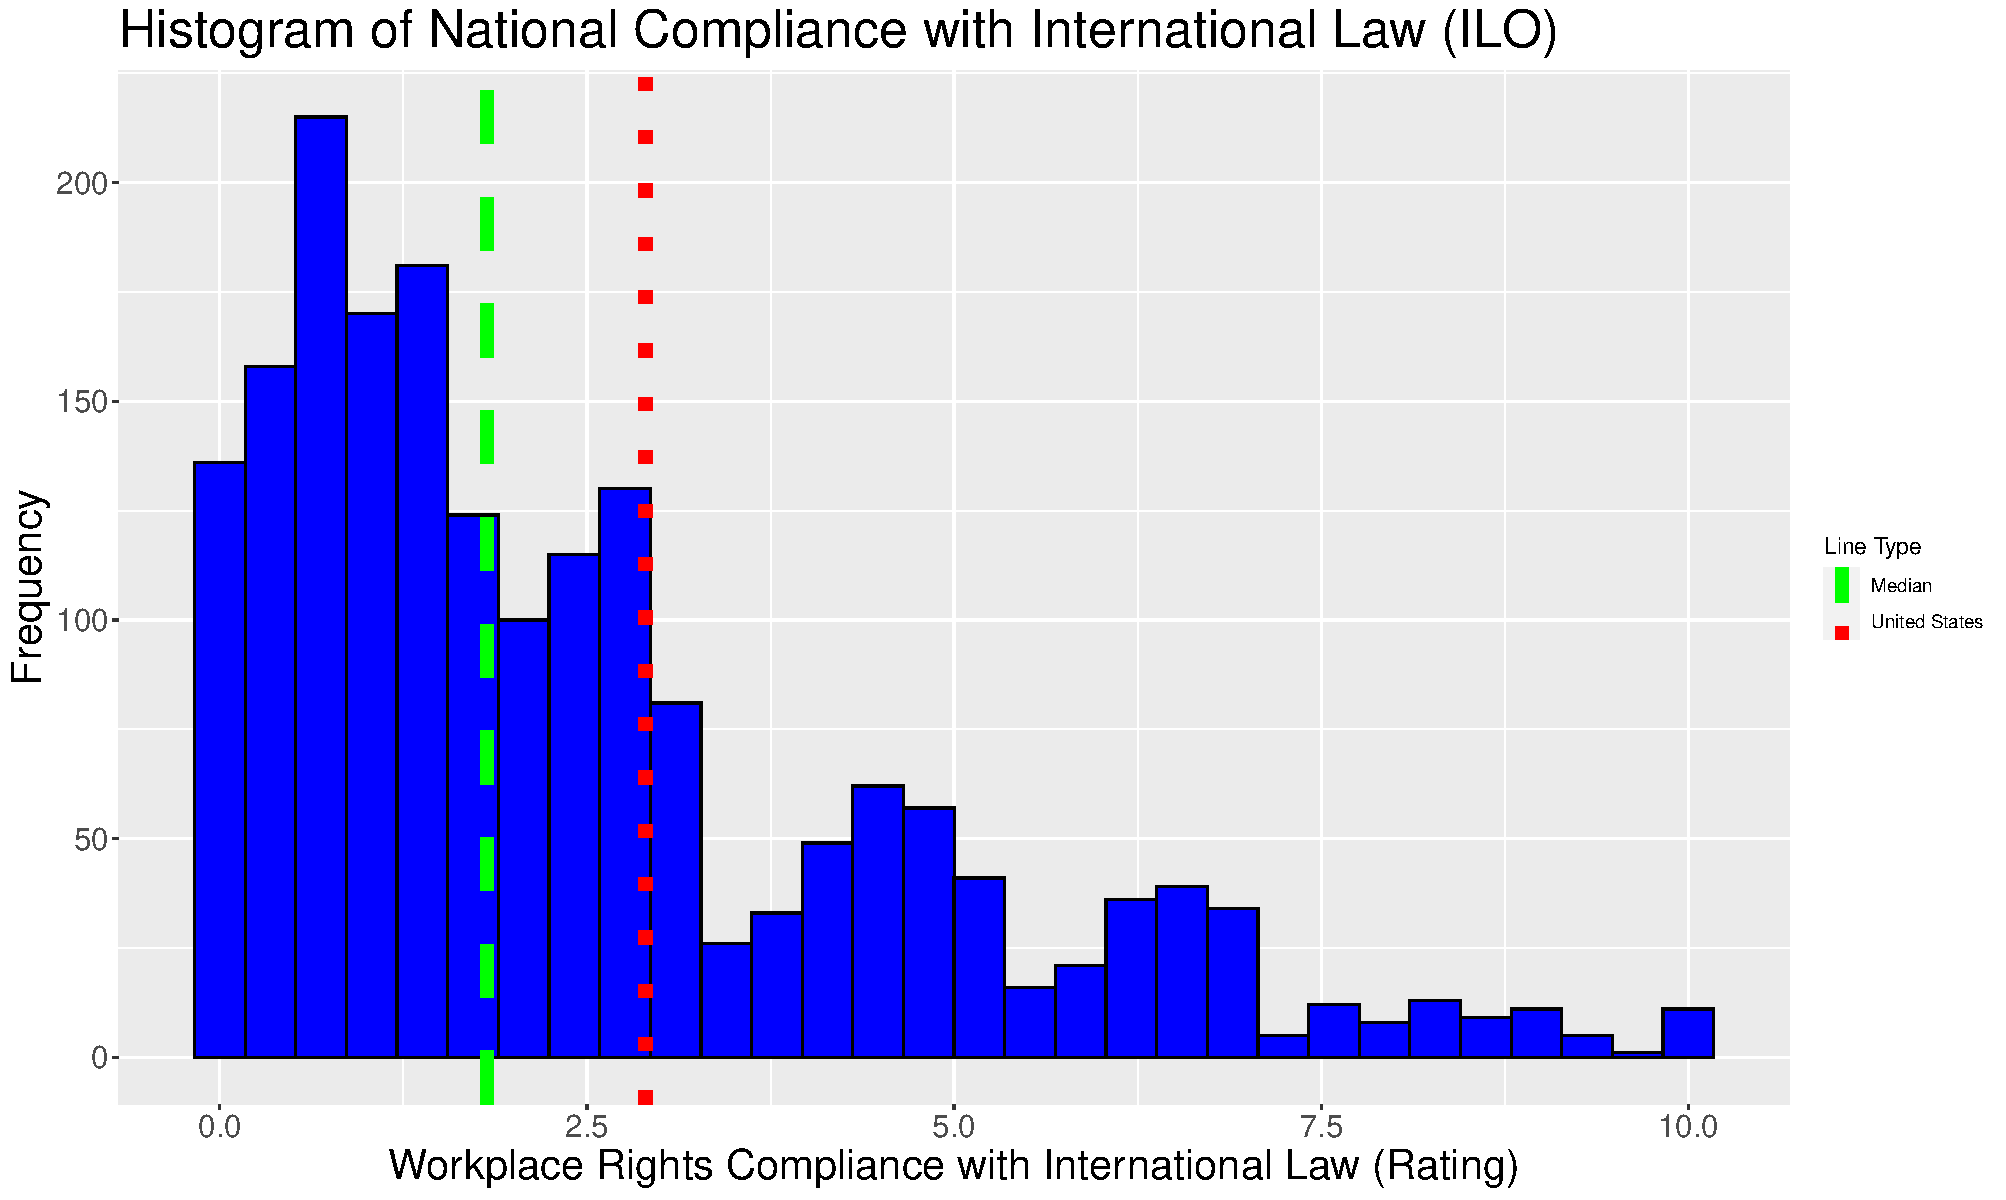
\includegraphics[width=.9\textwidth]{~/Lab2/graphs/plot_9.pdf}
  \caption{Histogram depicting the frequency distribution of Compliance with international law bargaining coverage as scale from 0 to 10 with 10 being the most out of compliance with international law a country could be, and 0 being completely incompliance with international labor law recorded by the International Labor organization. This data is grouped by country, the united states place is marked in the along with the mean of all countries.}
  \label{fig:2.3}
  \end{minipage}
\end{figure}

\clearpage
\section{Conclusion}
Summarize the main findings and their relevance to the initial objectives of your study.


\clearpage
\section{References}
\begin{enumerate}
    \item Visser, J. (2021). OECD/AIAS database on Institutional Characteristics of Trade Unions, Wage Setting, 
      State Intervention and Social Pacts (ICTWSS) [Data set]. OECD. 
      Retrieved from 
      \url{https://www.oecd.org/employment/ictwss-database.htm}
    \item International Labour Organization. (2022). Trade union density rate () 
      -- Annual (Id: ILR\_TUMT\_NOC\_RT\_A) [Data set]. Industrial Relations Data (IRdata). 
      Retrieved from 
      \url{https://www.ilo.org/shinyapps/bulkexplorer30/?lang=en\&id=ILR\_TUMT\_NOC\_RT\_A}
    \item International Labour Organization. (2022). Collective bargaining coverage 
      rate () -- Annual (Id: ILR\_CBCT\_NOC\_RT\_A) [Data set]. 
      Industrial Relations Data (IRdata). Retrieved from 
      \url{https://www.ilo.org/shinyapps/bulkexplorer36/?lang=en\&id=ILR\_CBCT\_NOC\_RT\_A}
    \item International Labour Organization. (2023). SDG indicator 8.8.2 - 
      Level of national compliance with labour rights
      (freedom of association and collective bargaining) 
      based on ILO textual sources and national legislation -- 
      Annual (Id: SDG\_0882\_NOC\_RT\_A) [Data set]. 
      SDG Labour Market Indicators (ILOSDG). Retrieved 
      from \url{https://www.ilo.org/shinyapps/bulkexplorer30/?lang=en\&id=ILR\_TUMT\_NOC\_RT\_A}
\end{enumerate}


\end{document}
